\documentclass[14pt]{extbook}
\usepackage{multicol, enumerate, enumitem, hyperref, color, soul, setspace, parskip, fancyhdr} %General Packages
\usepackage{amssymb, amsthm, amsmath, latexsym, units, mathtools} %Math Packages
\everymath{\displaystyle} %All math in Display Style
% Packages with additional options
\usepackage[headsep=0.5cm,headheight=12pt, left=1 in,right= 1 in,top= 1 in,bottom= 1 in]{geometry}
\usepackage[usenames,dvipsnames]{xcolor}
\usepackage{dashrule}  % Package to use the command below to create lines between items
\newcommand{\litem}[1]{\item#1\hspace*{-1cm}\rule{\textwidth}{0.4pt}}
\pagestyle{fancy}
\lhead{Progress Quiz 6}
\chead{}
\rhead{Version A}
\lfoot{9689-6866}
\cfoot{}
\rfoot{Spring 2021}
\begin{document}

\begin{enumerate}
\litem{
Evaluate the limit below, if possible.\[ \lim_{x \rightarrow 3} \frac{\sqrt{8x - 8} - 4}{9x - 27} \]\begin{enumerate}[label=\Alph*.]
\item \( \infty \)
\item \( 0.014 \)
\item \( 0.111 \)
\item \( 0.125 \)
\item \( \text{None of the above} \)

\end{enumerate} }
\litem{
Evaluate the one-sided limit of the function $f(x)$ below, if possible.\[ \lim_{x \rightarrow -4^+} \frac{6}{(x-4)^7}+8 \]\begin{enumerate}[label=\Alph*.]
\item \( -\infty \)
\item \( \infty \)
\item \( f(-4) \)
\item \( \text{The limit does not exist} \)
\item \( \text{None of the above} \)

\end{enumerate} }
\litem{
Based on the information below, which of the following statements is always true?
\begin{center}
    \textit{ $f(x)$ approaches $19.147$ as $x$ approaches $\infty$. }
\end{center}
\begin{enumerate}[label=\Alph*.]
\item \( f(x) \text{ is close to or exactly } \infty \text{ when } x \text{ is large enough}. \)
\item \( f(x) \text{ is close to or exactly } 19.147 \text{ when } x \text{ is large enough}. \)
\item \( x \text{ is undefined when } f(x) \text{ is large enough}. \)
\item \( f(x) \text{ is undefined when } x \text{ is large enough}. \)
\item \( \text{None of the above are always true.} \)

\end{enumerate} }
\litem{
Based on the information below, which of the following statements is always true?
\begin{center}
    \textit{ $f(x)$ approaches $2.934$ as $x$ approaches $2$. }
\end{center}
\begin{enumerate}[label=\Alph*.]
\item \( f(2) = 2 \)
\item \( f(2) \text{ is close to or exactly } 2 \)
\item \( f(2) = 2 \)
\item \( f(2) \text{ is close to or exactly } 2 \)
\item \( \text{None of the above are always true.} \)

\end{enumerate} }
\litem{
To estimate the one-sided limit of the function below as $x$ approaches 3 from the left, which of the following sets of numbers should you use?\[ \frac{\frac{3}{x} - 1}{x - 3} \]\begin{enumerate}[label=\Alph*.]
\item \( \{ 3.0000, 2.9000, 2.9900, 2.9990 \} \)
\item \( \{ 3.0000, 3.1000, 3.0100, 3.0010 \} \)
\item \( \{ 2.9000, 2.9900, 3.0100, 3.1000 \} \)
\item \( \{ 2.9000, 2.9900, 2.9990, 2.9999 \} \)
\item \( \{ 3.1000, 3.0100, 3.0010, 3.0001 \} \)

\end{enumerate} }
\litem{
Evaluate the limit below, if possible.\[ \lim_{x \rightarrow 4} \frac{\sqrt{7x - 12} - 4}{9x - 36} \]\begin{enumerate}[label=\Alph*.]
\item \( 0.097 \)
\item \( 0.014 \)
\item \( \infty \)
\item \( 0.125 \)
\item \( \text{None of the above} \)

\end{enumerate} }
\litem{
For the graph below, find the value(s) $a$ that makes the statement true: $ \displaystyle \lim_{x \rightarrow a} f(x)$ does not exist.
\begin{center}
    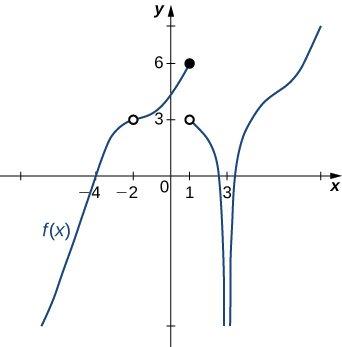
\includegraphics[width=0.5\textwidth]{../Figures/evaluateLimitGraphicallyCopyA.png}
\end{center}
\begin{enumerate}[label=\Alph*.]
\item \( 1 \)
\item \( -2 \)
\item \( 3 \)
\item \( \text{Multiple } a \text{ make the statement true}. \)
\item \( \text{No } a \text{ make the statement true}. \)

\end{enumerate} }
\litem{
For the graph below, find the value(s) $a$ that makes the statement true: $ \displaystyle \lim_{x \rightarrow a} f(x)$ does not exist.
\begin{center}
    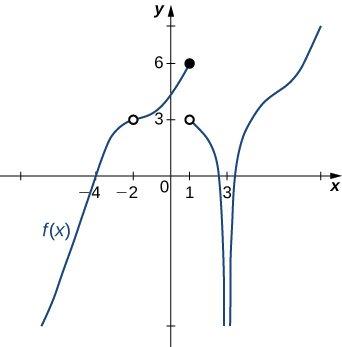
\includegraphics[width=0.5\textwidth]{../Figures/evaluateLimitGraphicallyA.png}
\end{center}
\begin{enumerate}[label=\Alph*.]
\item \( -2 \)
\item \( 1 \)
\item \( 3 \)
\item \( \text{Multiple } a \text{ make the statement true}. \)
\item \( \text{No } a \text{ make the statement true}. \)

\end{enumerate} }
\litem{
To estimate the one-sided limit of the function below as $x$ approaches 2 from the left, which of the following sets of numbers should you use?\[ \frac{\frac{2}{x} - 1}{x - 2} \]\begin{enumerate}[label=\Alph*.]
\item \( \{ 2.0000, 2.1000, 2.0100, 2.0010 \} \)
\item \( \{ 2.0000, 1.9000, 1.9900, 1.9990 \} \)
\item \( \{ 1.9000, 1.9900, 1.9990, 1.9999 \} \)
\item \( \{ 2.1000, 2.0100, 2.0010, 2.0001 \} \)
\item \( \{ 1.9000, 1.9900, 2.0100, 2.1000 \} \)

\end{enumerate} }
\litem{
Evaluate the one-sided limit of the function $f(x)$ below, if possible.\[ \lim_{x \rightarrow 5^-} \frac{-5}{(x-5)^8}+8 \]\begin{enumerate}[label=\Alph*.]
\item \( f(5) \)
\item \( \infty \)
\item \( -\infty \)
\item \( \text{The limit does not exist} \)
\item \( \text{None of the above} \)

\end{enumerate} }
\end{enumerate}

\end{document}